
\def\interminputs#1#2#3#4#5{
  ($(o) + (hgap)$) node[data] (det) {Detections #1}
  +(vgap) node[data] (pt) {Point Tracks #2}
  +($2*(vgap)$) node[data] (gp) {Ground plane #3}
  +($3*(vgap)$) node[data] (ego) {Egomotion #4}
  +($4*(vgap)$) node[data] (lane) {Lanes #5}
}

\newlength{\units}
\setlength{\units}{0.8cm}
\def\beginproblemflowchartsetup{
  \begin{tikzpicture}[
      every edge/.style = {very thick,>=stealth,draw,red,->},
      data/.style = {rectangle,rounded corners,fill=blue!20,draw,
      minimum width=3\units},
    algo/.style = {rectangle,fill=red!20,draw}]
    \coordinate (hgap) at (3.5, 0);
    \coordinate (vgap) at (0, -1);
    \coordinate (o) at (0,0);
   %\path[draw,use as bounding box] ($5*(vgap)-0.5*(hgap)$) rectangle ($-0.5*(vgap)+3*(hgap)$);
  }
\def\endproblemflowchartsetup{ \end{tikzpicture} }
\def\systemandout#1{
    \path 
    ($(o)+2*(vgap)+2*(hgap)$) node [algo] (os) {Our system}
    +($0.8*(hgap)$) node [data,align=left] (out) {3D localization\\ and dimensions #1};
}
\def\rawtointerm{
    \path (mv) edge (det);
    \path (mv) edge (pt);
    \path (mv) edge (gp);
    \path (mv) edge (ego);
    \path (mv) edge (lane);
    \path (gps) edge (lane);
    \path (map) edge (lane);
}
\def\intermtosys{
    \path (det) edge (os);
    \path (pt) edge (os);
    \path (gp) edge (os);
    \path (ego) edge (os);
    \path (lane) edge (os);

    \path (os) edge (out);
}
\newcommand{\problemflowchart}[5]{
  \beginproblemflowchartsetup
    \path 
    ($(o)+2*(vgap)$) node[data] (mv) {Mono-Video}
    ++($1.5*(vgap)$) node[data] (gps) {GPS}
    +($(vgap)$) node[data] (map) {Map};

    \path \interminputs{#1}{#2}{#3}{#4}{#5};

    \begin{pgfonlayer}{background}
      % Left-top corner of the background rectangle
      \path (det.east |- det.north)+(0.25,0.25) node (a) {};
      % Right-bottom corner of the background rectanle
      \path (mv.west |- map.south)+(-0.25,-0.25) node (c) {};
      % Draw the background
      \path[fill=green!20,rounded corners, draw=green,thick]
      (a) rectangle (c);
      \node at ($(det) - (hgap)$) {Inputs};
    \end{pgfonlayer}


    %\path[use as bounding box,draw] (map.south west) rectangle ($(out.east |- det.north)+(0.25,0.25)$);
    \systemandout{}

    \visible<2->{ 
      \path ($(out) - 2*(vgap) - (1cm, 0)$) node (ptvid) {
        \includemedia[label=pointtracks,
          width=5cm,
          activate=pageopen,
          addresource=graphics/pointtracksvideo.mp4,
          flashvars={
            source=graphics/pointtracksvideo.mp4
            &loop=true             % loop video
            &scaleMode=letterbox   % preserve aspect ratio while scaling the video
          }
        ]{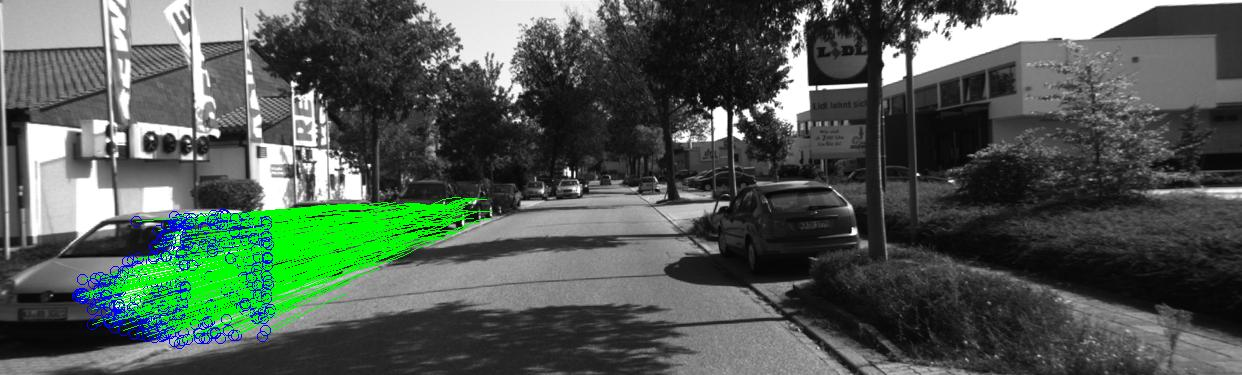
\includegraphics[width=\textwidth]{graphics/object_flow_tracks_4_000033.jpg}}{VPlayer.swf}
      };

      \draw[->,very thick,green!50!black] (pt) -- (ptvid);
    }

    \rawtointerm
    \intermtosys
  \endproblemflowchartsetup
}
\newcommand{\problemflowchartnoraw}[7]{
  \beginproblemflowchartsetup

    \path \interminputs{#1}{#2}{#3}{#4}{#5};

    \node (inp) at ($(det) - 0.8*(vgap)$) {Inputs #7};
    \begin{pgfonlayer}{background}
      % Left-top corner of the background rectangle
      \path (gp.east |- inp.north)+(0.25,0.25) node (a) {};
      % Right-bottom corner of the background rectanle
      \path (gp.west |- lane.south)+(-0.25,-0.25) node (c) {};
      % Draw the background
      \path[fill=green!20,rounded corners, draw=green,thick]
      (a) rectangle (c);
    \end{pgfonlayer}

    \systemandout{#6}

    \intermtosys

    \node [anchor=north west,align=left] (oseq) at ($(os)+2*(vgap)$) {\normalsize{$ \{\state{i}{t}\}^* = \arg \max_{\{\state{i}{t}\}} P(\{\state{i}{t}\} | \mathbb{E})\enspace. $}};
    \draw [->,very thick,green!50!black] (os) -- (oseq);
  \endproblemflowchartsetup
}
